% thermochem.tex

\section{Radiation transport}
\label{sec:radiation_transport}

The radiation source term in the Navier-Stokes equations (see Equation~\ref{eq:Q_rad}) is the negative divergence of the local radiative heat flux vector:

\begin{equation}
 - \nabla \cdot \vec{q}_\text{rad} = - \nabla \cdot \int_0^\infty \vec{I}_\nu d \nu \label{eq:div_q_rad}
\end{equation}

\noindent For application to computational grids it is convenient to express Equation~\ref{eq:div_q_rad} as the difference between the local emission and absorption:

\begin{equation}
- \nabla \cdot \vec{q}_\text{rad} =  \int^{\infty}_{0} \int_{4\pi} \kappa_{\nu} I_{\nu} d \omega d \nu - 4 \pi \int^{\infty}_{0} j_{\nu} d \nu
 \label{eq:divq_rad}
\end{equation}

A variety of models are implemented in Eilmer3  to solve for the radiative source term:

\begin{enumerate}
 \item Optically-thin model
 \item Tangent-slab model
 \item Modified Discrete Transfer model
 \item Photon Monte-Carlo model
\end{enumerate}

All models can be used on planar, axisymmetric or three-dimensional multi-block grids\footnote{The validity of the tangent-slab model, however, may be questionable when applied to certain geometrical configurations.}, and require the spectral emission $j_\nu$ and absorption $\kappa_\nu$ coefficients at each volume element and intensity $I_\nu$ emitted from each surface element as input.
Descriptions of these of models are provided in \textsection~\ref{sec:optically_thin} to~\ref{sec:photon_monte_carlo} respectively.
Firstly, however, the flowfield coupling methodology is outlined in the following section.

\subsection{Flowfield coupling}
\label{sec:fc}

As thermal radiation is approximately proportional to $T^4$, the effect of radiation on gasdynamic processes can be important for high temperature gases. 
A useful parameter for estimating the degree of radiation-flowfield coupling for blunt body flows is the Goulard number~\cite{goulard}:

\begin{equation}
 \Gamma = \frac{2 q_\text{rad}}{ \frac{1}{2} \rho_\infty u_\infty^3 }
\end{equation}

\noindent where $q_\text{rad}$ is the radiative heat flux incident at the stagnation point, $\rho_\infty$ the freestream density and $u_\infty$ the freestream velocity.
The Goulard number is a measure of the conversion of energy flux in the freestream to radiative energy flux at the vehicle surface.
When the Goulard number becomes large ($\Gamma > 0.01$) radiation-flowfield coupling should be taken into consideration due to significant levels of radiative flux through the shock layer.

\par

As the radiation transport procedure is computationally expensive, it is desirable to update the radiation source terms at a reasonably low frequency (\textit{i.e.} a \textit{loosely} coupled approach).
When a radiation transport calculation at time-step $n$ is performed, $\rho$, $T_{e}$ and $\nabla \cdot \vec{q}_\text{rad}$ for each cell are stored\footnote{When a one temperature gas-model is used, $T_e = T$.}.
For each of the subsequent flowfield time-steps $m$ where a complete radiation transport calculation is not performed the radiative divergence is rescaled to account for variations in the gas-state:

\begin{equation}
 \left ( - \nabla \cdot \vec{q}_\text{rad} \right )_m = \left \lbrace \begin{array}{c} \frac{ \left ( \rho T_{e}^{4} \right )_{m} }{ \left ( \rho T_{e}^{4} \right )_{n} } \left ( - \nabla \cdot \vec{q}_\text{rad} \right )_n \text{ \hspace{0.6cm} for } \left ( - \nabla \cdot \vec{q}_\text{rad} \right )_n > 0 \\ \\  \frac{ \left ( \rho T_{e}^{-4} \right )_{m} }{ \left ( \rho T_{e}^{-4} \right )_{n} } \left ( - \nabla \cdot \vec{q}_\text{rad} \right)_n \text{ \hspace{0.6cm} for } \left ( - \nabla \cdot \vec{q}_\text{rad} \right )_n < 0 \end{array} \right .
 \label{eq:divq_scale}
\end{equation}

The frequency of the radiation update is dependent on the transient behavior of the flowfield;  for example, during the initial period of flow development the update frequency needs to be high to account for shifting shock positions, while as the solution approaches steady state the update frequency can be substantially reduced.

\subsection{Optically-thin model}
\label{sec:optically_thin}

The optically-thin model neglects reabsorption, reducing Eq.~\ref{eq:divq_rad} to:

\begin{equation}
 - \nabla \cdot \vec{q}_\text{rad} = - 4 \pi \int^{\infty}_{0} j_{\nu} d \nu \label{eq:divq_rad_OT}
\end{equation}

\noindent The radiative divergence therefore becomes a function of the local gas state only.
This is a good model to use when emission is much higher than absorption, as the effect of radiation-flowfield coupling can then by modelled with minimum computational effort.

\subsection{Tangent-slab model}
\label{sec:TS_model}

The tangent-slab model allows the effect of reabsorption to be modelled while avoiding a complete directional integration of the local intensity field.
A one-dimensional variation of properties is considered along each line-of-sight normal to the vehicle surface.
Computationally, a line of cells is used to represent the normal line-of-sight as demonstrated in Figure~\ref{fig:FireII-TS}.
If a single column of blocks is used to define the computational domain-between the inflow and vehicle surface boundaries, the tangent-slab model is inherently parallelisable as all the information required for the calculation is contained in the local block.

\par

\begin{figure}[h]
 \center
 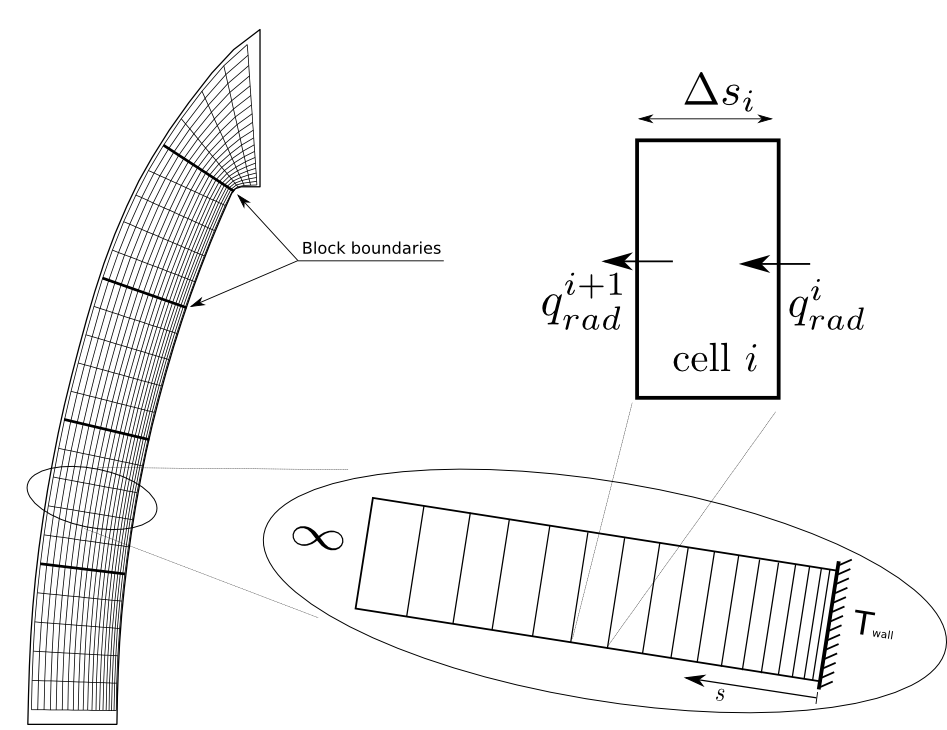
\includegraphics[scale=0.85]{radiation/figures/FireII-TS.png}
 \caption{Schematic of tangent-slab calculation domain along lines of cells on a multi-block grid.}
 \label{fig:FireII-TS}
\end{figure} 

Given that the infinite-slab arrangement will result in zero net radiative flux in the transverse directions, the definition of the radiative divergence for slab $i$ reduces to:

\begin{equation}
 - \left( \nabla \cdot \vec{q}_\text{rad} \right )_{i} = - \left ( \frac{\partial q_\text{rad}}{\partial s} \right )_{i} \approx \frac{ - \left ( q_\text{rad}^{(i+1)} - q_\text{rad}^{(i)} \right ) }{ \Delta s_{i} }
 \label{eq:divq_TS}
\end{equation}

\noindent where $q_{rad}^{(i)}$ is the radiative flux at the $i^{th}$ cell interface (\textit{i.e.} preceeding the cell from right-to-left) and $\Delta s_{i}$ is the width of the cell in the (approximately) body normal direction.
The solution for the radiative flux in a gaseous medium between two parallel, infinite-slabs as a function of the spectral optical thickness $\tau_{\nu}$ is derived in the text by Modest~\cite{Mod03}.
If the computational domain is considered to be a collection of $N_\text{slabs}$ isothermal slabs with the spectral range discretised into $N_\nu$ frequency intervals the radiative flux at interface $i$ can be expressed as:

\begin{equation}
 q_\text{rad}^{(i)} = \sum_{k=1}^{N_\nu} 2 \pi I_{\nu_k, \text{wall}} E_{3} \left ( \tau_{\nu_k}^{(i)} \right ) + 2 \pi \sum_{j=1}^{N_{\text{slabs}}} S_{\nu_k}^{(j)} \left [ E_{3} \left ( \left  | \tau_{\nu_k}^{(i)} - \tau_{\nu_k}^{(j)} \right  | \right ) - E_{3} \left ( \left  | \tau_{\nu_k}^{(i)} - \tau_{\nu_k}^{(j-1)} \right  | \right ) \right ] \Delta \nu_k
 \label{eq:TS_modest}
\end{equation}

\noindent where $S_{\nu_k}^{(i)}$ is the source function for the $i^{th}$ isothermal cell at frequency $\nu_k$, $I_{\nu_k, \text{wall}}$ is the intensity emitted by the wall and the optical thickness $\tau_{\nu_k}^{(i)}$ is calculated as:

\begin{equation}
 \tau_{\nu_k}^{(i)} = \sum_{l=1}^{i} \kappa_{\nu_k}^{(l)} \Delta s_{l}
 \label{eq:tau_nu}
\end{equation}

\noindent The $E_{n}$ term is the $n^\text{th}$ order exponential integral with form:

\begin{equation}
 E_{n} ( x ) = \int_{1}^{\infty} \omega^{-n} \text{exp} \left ( - \omega x \right ) d \omega
 \label{eq:E_n}
\end{equation}

\noindent The $E_{3}$ curve fit derived  by Johnston~\cite{JohnPhd} is implemented for the Eilmer3  tangent-slab model:

\begin{equation}
 E_{3} ( x ) = 0.0929 e^{-4.08x} + 0.4071e^{-1.33x}
 \label{eq:E3}
\end{equation}

\noindent The intensity emitted by the wall with emissivity $\epsilon_{\text{wall}}$ is calculated as~\cite{VK65}:

\begin{equation}
 I_{\nu, \text{wall}} = 2 \pi \epsilon_{\text{wall}} \sigma T_{\text{wall}}^{4}
 \label{eq:qwall}
\end{equation}

\noindent where $T_{\text{wall}}$ is the blackbody wall temperature.  

\subsection{Modified discrete transfer model}
\label{sec:discrete_transfer}

A modified version of the standard discrete transfer model~\cite{shah, elbert_cinnella, karl2001} has been implemented in the \texttt{Eilmer3}  framework.
This is a ray-tracing based model, where the radiative divergence and heat-fluxes are determined by direct numerical integration of the radiant energy field over direction and space via the generation of a `radiation sub-grid' mapped over the CFD grid.
The radiation sub-grid consists of rays distributed isodirectionally from each emitting element in the flowfield, with the flow state and radiation spectra defined at distributed points along each ray.
An example of a radiation sub-grid on a simple axisymmetric CFD grid is illustrated in Figure~\ref{fig:radiation-subgrid}.
Although the modified discrete transfer model has been implemented in Eilmer3  for planar, axisymmetric and 3D geometries, only the planar and axisymmetric formulations are described herein.

\begin{figure}[h]
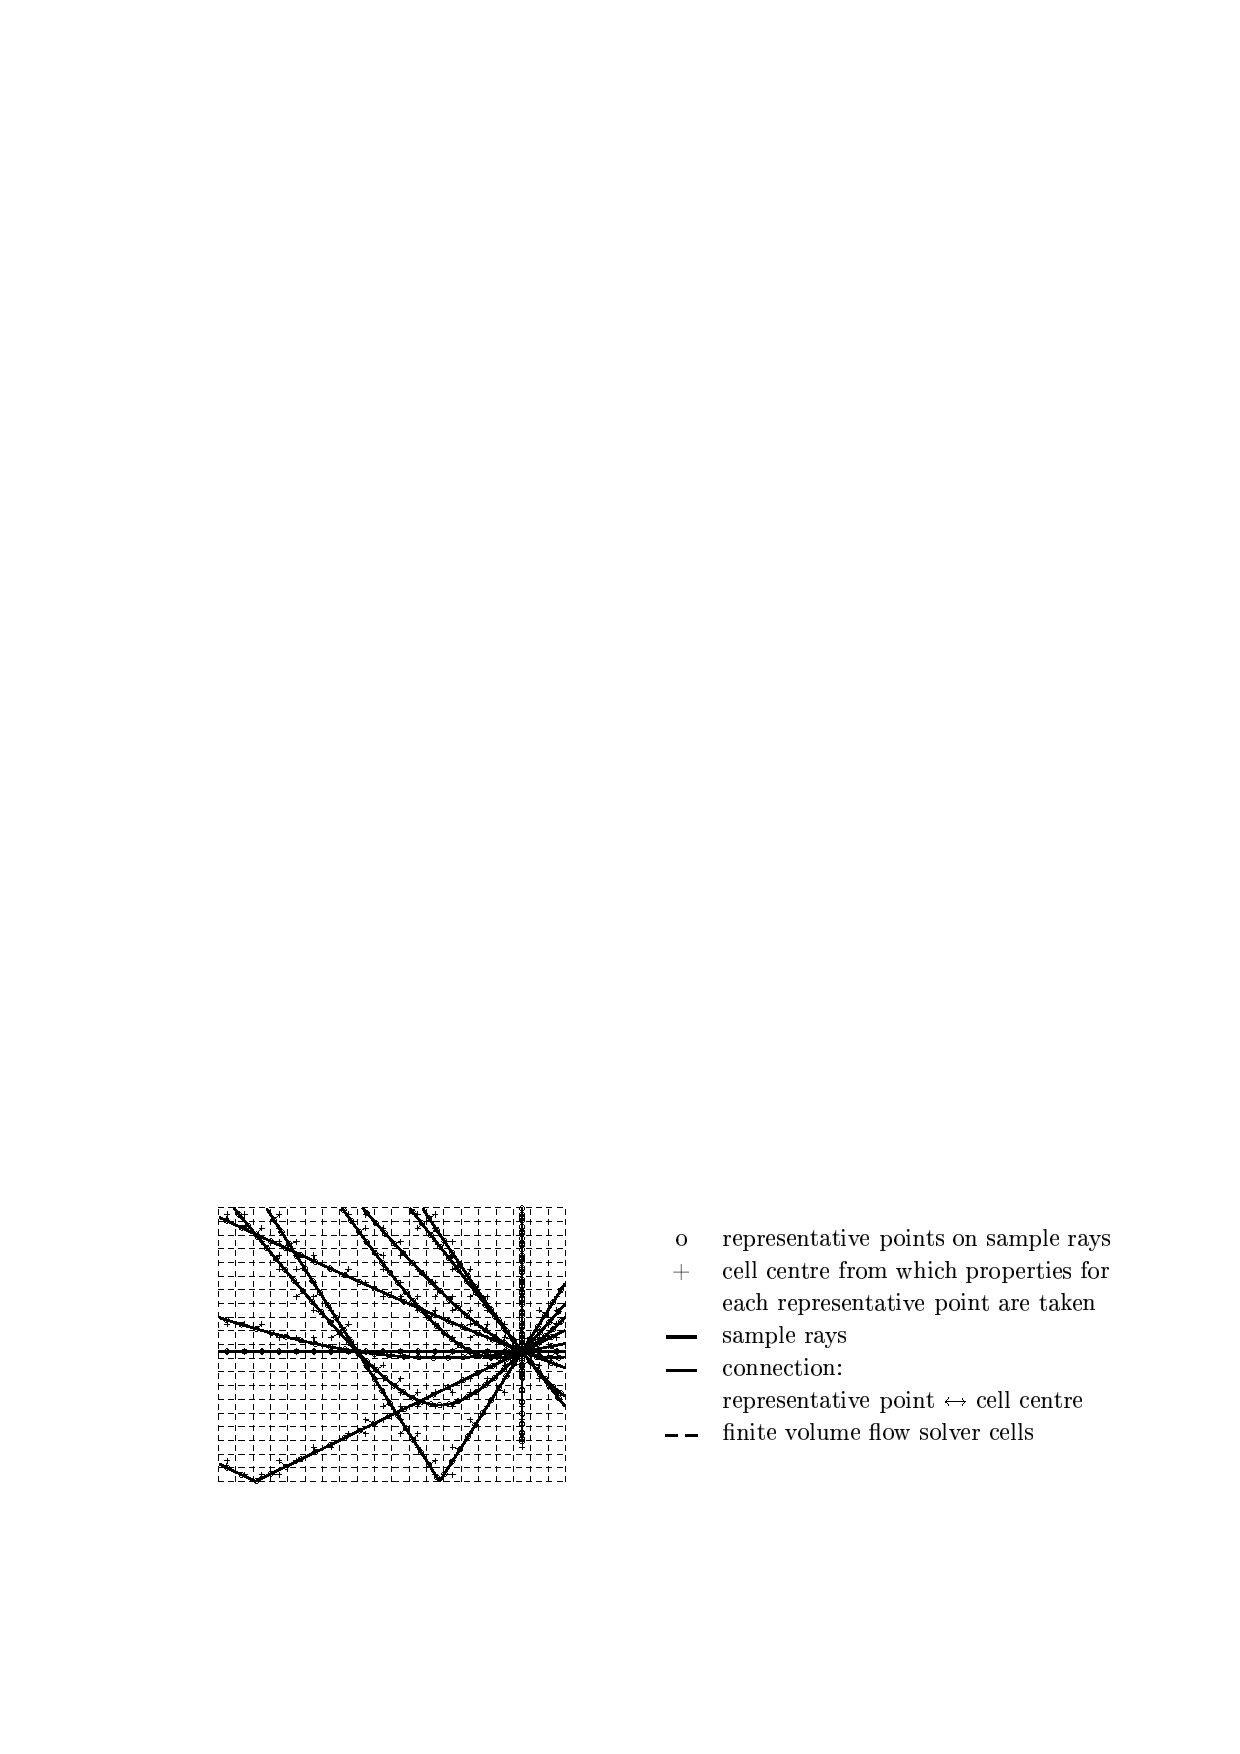
\includegraphics[width=\linewidth]{radiation/figures/axi-radiation-subgrid.pdf}
 \caption{Example radiation sub-grid on a simple axisymmetric grid (Reference~\cite{karl2001}).}
 \label{fig:radiation-subgrid}
\end{figure}

\par

The Discrete Transfer model proposed by Elbert and Cinella~\cite{elbert_cinnella} uses the radiation sub-grid to solve directly for the radiative divergence via Eq.~\ref{eq:divq_rad}.
The modified Discrete Transfer model method proposed by Karl~\cite{karl2001} uses the radiation sub-grid to solve for the heat flux vectors throughout the flowfield, from which the divergence at the cell centres can be calculated.
In contrast, the modified Discrete Transfer model implemented in \texttt{Eilmer3} uses the radiative sub-grid to transport packets of radiant energy through the computational domain.
This is similar to a photon Monte-Carlo method in that radiation is treated as a discrete quantity rather than a continuous field, however the ray-distribution is kept uniform and energy attenuation is not modelled in a statistical fashion.

\subsubsection{Governing equations}

The total radiative divergence for a finite-volume cell is calculated as the difference between the total emissive power $E_{\text{ems.}}$ and absorptive power $E_{\text{abs.}}$ divided by the cell volume $V$:

\begin{equation}
 - \nabla \cdot \vec{q}_\text{rad} = \frac{ - \left ( E_{\text{ems.}} - E_{\text{abs.}} \right ) }{V}
 \label{eq:my_divq}
\end{equation}

\noindent where:

\begin{eqnarray}
 E_{\text{ems.}} &=& \int_{V} \int_{0}^{{4\pi}} \int_{\nu_{\text{min}}}^{\nu_{\text{max}}} j_{\nu} d\nu d\omega dV = \sum_{r}^{N_{\text{ems. rays}}} \sum_{n}^{N_{\nu}} E_{r,n}^0 \label{eq:E_emission} \\
 E_{\text{abs.}} &=& \sum_{r}^{N_{\text{abs. rays}}} \sum_{n}^{N_{\nu}} \left ( - \Delta E_{r,n} \right ) \label{eq:E_absorption} 
\end{eqnarray}

\noindent Here $N_{\text{abs. rays}}$ is the total number of ray segments traversing the current cell, $N_{\text{ems. rays}}$ is the total number of rays emitted by this cell and the frequency domain has been divided into $N_{\nu}$ intervals between $\nu_{min}$ and $\nu_{max}$. 
$E_{r,n}^0$ is the initial power carried by photon packet $n$ with frequency interval $\Delta \nu_{n}$ from ray $r$ with solid angle $\Delta \omega_{r}$:

\begin{equation}
 E_{r,n}^0 = j_{\nu} \Delta \nu_{n} \Delta \omega_{r} V
\end{equation}

The radiative heat flux incident on wall elements $q_\text{rad}$ is calculated as the sum of the remaining energy $E_{r,n}$ from all incident rays $N_\text{inc. rays}$ divided by the wall element area $A$:

\begin{equation}
 q_\text{rad} = \frac{ E_\text{abs.} }{A} =  \frac{ \displaystyle \sum_{r}^{N_{\text{inc. rays}}} \displaystyle \sum_{p}^{N_{\nu}} E_{r,n} }{ A }
 \label{eq:my_divq}
\end{equation}

\noindent Note that all surfaces are currently treated as blackbodies, and therefore reflection is not considered.

\subsubsection{Absorption model}

The radiative power lost by photon packet $p$ while traversing from points $s_{i}$ to $s_{f}$ along a ray is calculated from Beers law:

\begin{equation}
 - \Delta E_{r,n} = - ( 1 - e^{-\kappa_{\nu_{n}}(s) \Delta s } ) E_{r,n}(s_{i})
 \label{eq:E_rn}
\end{equation}

\noindent where $\Delta s = s_{f} - s_{i}$.

\subsubsection{Determination of ray density distribution}
\label{sec:ray_density_distribution}

A number of approaches are implemented for determining the number of rays emitted from each volume element, $N_{\text{ems. rays}}$:

\begin{description}
 \item[No clustering] All elements emit the same number of photons
 \item[Area clustering] The number of emitted photons for each element is proportional to the total radiative power density times area (2D grids only)
 \item[Volume clustering] The number of emitted photons for each element is proportional to the total radiative power density times volume (2D and 3D grids)
\end{description}

\noindent The area and volume clustering approaches allow more rays to be emitted from elements emitting more radiation, resulting in each ray in the calculation handling approximately the same energy.
The area clustering approach is included to avoid the problem of very small cell volumes near the axis of symmetry for axisymmetric grids.
The number of rays emitted from a volume element $i$ via the area clustering approach is:

 \begin{equation}
 N_{i} = \text{int} \left [ N_{\text{max}} \frac{ e_{i} A_i }{ \text{max}_i ( e_{i} A_i ) } \right ] \label{eq:N_photons}
\end{equation}

\noindent where $N_{\text{max}}$ is the maximum permitted number of rays, $e_{i}$ is the total radiative power density from volume element $i$ and $A_i$ is the area of element $i$.
The total radiative power density for volume element $i$ is calculated as:

\begin{equation}
 e_i = \int_{\nu_{\text{min}}}^{\nu_{\text{max}}} j_{\nu,i} d \nu
\end{equation}

Similarly, the number of photons emitted from a volume element $i$ via the volume clustering approach is:

 \begin{equation}
 N_{i} = \text{int} \left [ N_{\text{max}} \frac{ e_{i} V_i }{ \text{max}_i ( e_{i} V_i ) } \right ] \label{eq:N_photons}
\end{equation}

\noindent where $V_i$ is the volume of volume element $i$.
Analogous expressions are implemented for determining the number of rays emitted from surface elements, where length and area weightings are used in place of area and volume.

\subsubsection{Radiation sub-grid}
\label{sec:radiation_subgrid}

The radiation sub-grid for planar and axisymmetric grids of quadrilateral cells described by Elbert and Cinella~\cite{elbert_cinnella} and Karl~\cite{karl2001} is implemented with slight modifications.
The radiation sub-grid coordinates of a point at distance $L$ along a ray with elevation and azimuth angles $\phi$ and $\theta$ originating from position $x_0$, $y_0$ are:

\begin{eqnarray}
 x' &=& x_0 + L \text{cos} \left ( \phi \right ) \text{cos} \left ( \theta \right ) \\
 y' &=& y_0 + L \text{sin} \left ( \phi \right ) \\
 z' &=& L \text{cos} \left ( \phi \right ) \text{sin} \left ( \theta \right )
\end{eqnarray}

\noindent For 2D calculations, the corresponding CFD grid coordinates are then calculated from the following transformation:

\begin{eqnarray}
 x &=& x' \\
 y &=& \sqrt{y'^2 + z'^2}
\end{eqnarray}

\noindent This transformation has the effect of reflecting rays intersecting the symmetry axis at $y=0$, as required (see Figure~\ref{fig:radiation-subgrid}).
For planar geometries the radiation sub-grid is formed in the $x$--$y$ plane as the CFD domain is symmetrical along the $z$ axis.
For ray $i$ of $N_\text{rays}$ the elevation and azimuth angles are calculated as:

\begin{eqnarray}
 \theta &=& \left \lbrace \begin{array}{ccc} 0 & \text{for} & 0 \leq \alpha < \pi/2  \\ 
 									    \pi & \text{for} & \pi/2 \leq \alpha < 3\pi/2 \\
									     0 & \text{for} & 3\pi/2 \leq \alpha < 2\pi \end{array} \right . \\
 \phi &=& \left \lbrace \begin{array}{ccc} \alpha & \text{for} & 0 \leq \alpha < \pi/2  \\ 
 									    \pi - \alpha & \text{for} & \pi/2 \leq \alpha < 3\pi/2 \\
									     \alpha - \pi/2 & \text{for} & 3\pi/2 \leq \alpha < 2\pi \end{array} \right .
\end{eqnarray}

\noindent where  $\alpha = i \frac{2\pi}{N_\text{rays}}$.
For axisymmetric geometries the radiation sub-grid must be formed in three-dimensions as the CFD domain is radially symmetrical about $y=0$.
Elbert and Cinella~\cite{elbert_cinnella} and Karl~\cite{karl2001} use the symmetric vertices of the icosahedron platonic solid to generate the axisymmetric elevation and azimuth angles.
This approach, however, limits the total number of rays to a set of fixed values as the 20 icosahedron faces must be subdivided equally to achieve approximate uniformity.
To allow for an arbitrary number of axisymmetric rays, the so-called `Golden Section Spiral' method~\cite{Spiral} of generating uniform points on a sphere has been implemented.
As illustrated in Figure~\ref{fig:gspirals}, this method arranges nodes on the surface of a unit sphere by considering spirals with successive longitudes chosen according to the golden ratio $\frac{\sqrt{5}-1}{2}$.

\begin{figure}[h]
\centering
\subfloat[$N_{rays} = 23$]{\scalebox{0.9}{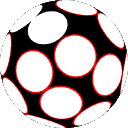
\includegraphics{radiation/figures/golden_spiral-A.png}}} \hspace{0.2cm}
\subfloat[$N_{rays} = 133$]{\scalebox{0.9}{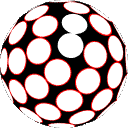
\includegraphics{radiation/figures/golden_spiral-B.png}}} \hspace{0.2cm}
\subfloat[$N_{rays} = 480$]{\scalebox{0.9}{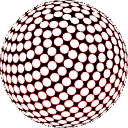
\includegraphics{radiation/figures/golden_spiral-C.png}}}
\caption{Approximately uniform points on a sphere generated via the `Golden Section Spiral' method~\cite{Spiral}.}
\label{fig:gspirals}
\end{figure}

The unit sphere coordinates of ray $i$ of $N_\text{rays}$ are calculated as:

\begin{eqnarray}
 x^\ast &=& r \text{cos}(\alpha) \\
 y^\ast &=& w \\
 z^\ast &=& r \text{sin}(\alpha)
\end{eqnarray}

\noindent where:

\begin{eqnarray}
 w &=& i \frac{2}{N_\text{rays}} - 1 + N_\text{rays} \\
 r &=& \sqrt{ 1 - w^2 } \\
 \alpha &=& i \pi ( 3 - \sqrt{5} )
\end{eqnarray}


\noindent The elevation and azimuth angles are then calculated as:

\begin{eqnarray}
 \phi &=& \text{arcsin} \left ( y^\ast \right ) \\
 \theta &=& \left \lbrace \begin{array}{ccccc} \text{arctan} \left ( \frac{z^\ast}{x^\ast} \right ) & \text{ for } & x^\ast > 0 & \text{and} & z^\ast > 0 \\
 										  \pi / 2                                                                 & \text{ for } & x^\ast = 0 & \text{and} & z^\ast > 0 \\
  										  \pi - \text{arctan} \left ( \frac{z^\ast}{-x^\ast} \right ) & \text{ for } & x^\ast < 0 & \text{and} & z^\ast > 0 \\ 
										  \pi                                                                      & \text{ for } & x^\ast < 0 & \text{and} & z^\ast = 0 \\
										  \pi + \text{arctan} \left ( \frac{-z^\ast}{x^\ast} \right ) & \text{ for } & x^\ast < 0 & \text{and} & z^\ast < 0 \\ 
										  3 \pi / 2                                                              & \text{ for } & x^\ast = 0 & \text{and} & z^\ast < 0 \\ 
										  2\pi - \text{arctan} \left ( \frac{-z^\ast}{x^\ast} \right ) & \text{ for } & x^\ast > 0 & \text{and} & z^\ast < 0 \\
										  0                                                                        & \text{ for } & x^\ast > 0 & \text{and} & z^\ast = 0 \\ \end{array} \right .
\end{eqnarray}

\noindent The angular distribution of the rays for this method is not as uniform as that for the subdivided icosahedron approach, however the ray number flexibility is a distinct advantage.

\subsubsection{Ray-tracing}
\label{sec:ray_tracing}

The core of the ray-tracing method are cell searching algorithms that allows the radiation sub-grid to be mapped onto the CFD grid, Figure~\ref{fig:cell-searching}.
Given the coordinates of a point along a ray, these algorithms solve for what cell this point lies in.

\begin{figure}[h]
 \centering
 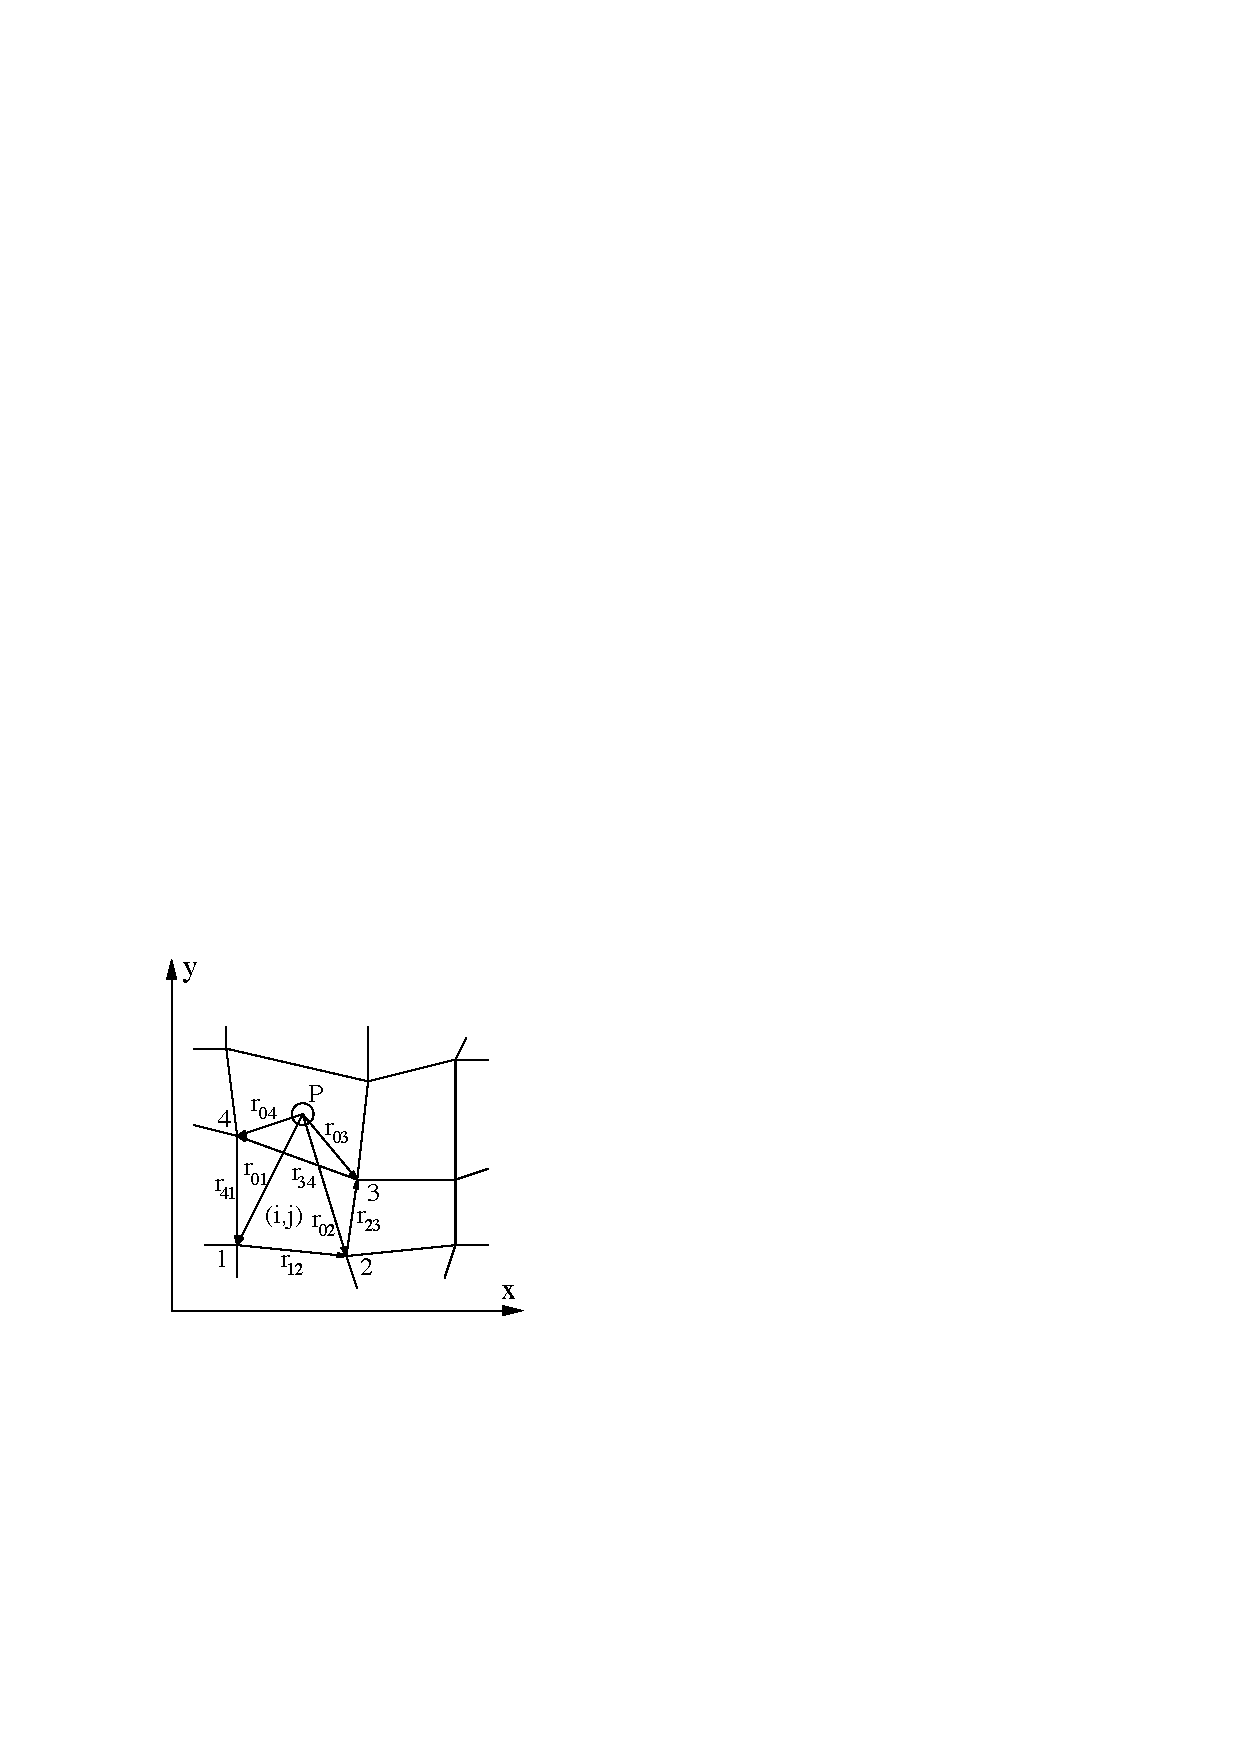
\includegraphics[width=0.5\linewidth]{radiation/figures/cell_searching.pdf}
 \caption{Mapping of the radiation sub-grid onto the CFD grid, Reference~\cite{karl2001}.}
 \label{fig:cell-searching}
\end{figure}

\paragraph{Two dimensional grids}

For a given trial cell with indices $i$ and $j$ the following cross-products are evaluated:

\begin{eqnarray}
  a_{12} \cdot \vec{n} &=& \vec{r}_{01} \times \vec{r}_{12} \\
  a_{23} \cdot \vec{n} &=& \vec{r}_{02} \times \vec{r}_{23} \\
  a_{34} \cdot \vec{n} &=& \vec{r}_{03} \times \vec{r}_{34} \\
  a_{41} \cdot \vec{n} &=& \vec{r}_{04} \times \vec{r}_{41}
\end{eqnarray}

\noindent where $\vec{n}$ is the unit vector normal to the x-y plane.
If all four cross-products are positive the point $p$ is inside the trial cell.
Otherwise, the indices of the next trial cell are obtained according to:

\begin{eqnarray}
 \text{if } \left ( a_{23} < 0 \text{ and } a_{41} > 0 \right ) \text{ then } i = i + 1 \\ 
 \text{if } \left ( a_{23} > 0 \text{ and } a_{41} < 0 \right ) \text{ then } i = i - 1 \\
 \text{if } \left ( a_{12} < 0 \text{ and } a_{34} > 0 \right ) \text{ then } j = j + 1 \\
 \text{if } \left ( a_{12} > 0 \text{ and } a_{34} < 0 \right ) \text{ then } j = j - 1 
\end{eqnarray}

\paragraph{Three dimensional grids}

For a given trial hexahedral cell with indices $i$, $j$ and $k$ the following product is evaluated for each face:

\begin{equation}
 a = \vec{v}_1 \cdot \left ( \vec{v}_2 \times \vec{v}_3 \right )
\end{equation}

\noindent where $\vec{v}_1$, $\vec{v}_2$ and $\vec{v}_3$ are any three consecutive vertices in the clockwise direction (observed from the exterior of the cell) of the four vertices forming the face.
The sign of $a$ determines which side of the face the point lies.
If all $a$ values are negative, the point is inside the cell.
Otherwise, the indices of the next trial cell are obtained according to:

\begin{eqnarray}
 \text{if } \left ( a_\text{east} > 0 \text{ and } a_\text{west} < 0 \right ) \text{ then } i = i + 1 \\ 
 \text{if } \left ( a_\text{east} < 0 \text{ and } a_\text{west} > 0 \right ) \text{ then } i = i - 1 \\ 
 \text{if } \left ( a_\text{north} > 0 \text{ and } a_\text{south} < 0 \right ) \text{ then } j = j + 1 \\ 
 \text{if } \left ( a_\text{north} < 0 \text{ and } a_\text{south} > 0 \right ) \text{ then } j = j - 1 \\ 
 \text{if } \left ( a_\text{top} > 0 \text{ and } a_\text{bottom} < 0 \right ) \text{ then } k = k + 1 \\ 
 \text{if } \left ( a_\text{top} < 0 \text{ and } a_\text{bottom} > 0 \right ) \text{ then } k = k - 1 
\end{eqnarray}

\noindent As the mapping of the radiation sub-grid is performed successively for each point along a ray, a good initial guess is always available and the above methods are highly efficient.

\subsubsection{Solution procedure}

The procedure for calculating the radiative divergence field and heat flux profiles in Eilmer3  with the modified Discrete Transfer model is as described in Figure~\ref{fig:eilmer-DT-solve-procedure}.
Note that the frequency range is able to be divided up into multiple blocks, allowing the total memory requirement for the calculation to be reduced.
This is necessary when the CFD and spectral grids are vey fine.

\begin{figure}[htbp]
\small
\begin{center}
\fbox{\parbox{13cm}{
 \begin{enumerate}
  \item Perform geometric ray-tracing to define the radiation sub-grid
  \item Calculate emission and absorption spectra for each cell and wall element
  \item Trace each photon packet through the grid
  \begin{enumerate}
   \item Subtract emitted energy from origin cell
   \item Add absorbed energy to each traversed cell
   \item Record exiting energy on wall elements 
  \end{enumerate}
  \item Evaluate $- \nabla \cdot \vec{q}_\text{rad}$ for each cell and $q_\text{rad}$ for each wall element from the results
  \item Repeat steps 2 - 4 for each frequency block
 \end{enumerate}
}}
\end{center}
\caption{Sequence of operations for calculating the radiative divergence field and heat flux profiles in \texttt{Eilmer3} with the modified Discrete Transfer model.}
\label{fig:eilmer-DT-solve-procedure}
\end{figure}

This procedure is parallelised via \verb OpenMP  where each processor has access to all data describing the computational domain.
The calculation is divided amongst the available processors on a cell-by-cell basis when computing spectra, and a ray-by-ray basis when tracing and integrating along lines-of-sight.

\subsection{Photon Monte-Carlo model}
\label{sec:photon_monte_carlo}

A photon Monte-Carlo model based on the model described by Wang and Modest~\cite{WM2007} has been implemented in \texttt{Eilmer3}.
Both line-by-line and gray gas spectral models can be considered.
This model is similar to the modified Discrete Transfer model described in the previous section in that a ray-tracing approach is used.
The Monte-Carlo approach, however, treats the emission and absorption of photons in a statistical manner and has the advantage of being easily adapted to flowfields with strongly varying gas properties.

\subsubsection{Governing equations}

The total radiative divergence for a finite-volume cell is calculated as the difference between the total emissive power $E_{\text{ems.}}$ and absorptive power $E_{\text{abs.}}$ divided by the cell volume $V$:

\begin{equation}
 - \nabla \cdot \vec{q}_\text{rad} = \frac{ - \left ( E_{\text{ems.}} - E_{\text{abs.}} \right ) }{V}
 \label{eq:my_divq}
\end{equation}

\noindent where:

\begin{eqnarray}
 E_{\text{ems.}} &=& \int_{V} \int_{0}^{{4\pi}} \int_{\nu_{\text{min}}}^{\nu_{\text{max}}} j_{\nu} d\nu d\omega dV = \sum_{p}^{N_{\text{ems. photons}}} E_{p}^0 \label{eq:E_emission} \\
 E_{\text{abs.}} &=& \sum_{p}^{N_{\text{abs. photons}}} \left ( - \Delta E_{p} \right ) \label{eq:E_absorption} 
\end{eqnarray}

\noindent Here $N_{\text{abs. photons}}$ is the total number of photon packets with energy being absorbed by the current cell and $N_{\text{ems. photons}}$ is the total number of photons emitted by this cell.
$E_{p}^0$ is the initial power carried by photon packet $p$:

\begin{equation}
 E_{p}^0 = \frac{ 4 \pi V  }{ N_{\text{ems. photons} } } \int_{\nu_{\text{min}}}^{\nu_{\text{max}}} j_{\nu} d \nu
\end{equation}

The absorption of radiation by walls is modelled probabilistically.  An incident photon is absorbed if a uniform random number is less than or equal to the surface emissivity:

\begin{equation}
R_\text{abs.} \leq \epsilon_\text{wall}
\end{equation}

\noindent and undergoes diffuse reflection otherwise.
This results in 100\% absorption for walls with an emissivity of 1 and no absorption for walls with an emissivity of 0, as required.
The radiative heating of wall elements $q_\text{rad}$ is then calculated as the sum of the remaining energy $E_{p}$ from all incident photons $N_\text{inc. photons}$ divided by the wall element area $A$:

\begin{equation}
 q_\text{rad} = \frac{ E_\text{abs.} }{A} =  \frac{ \displaystyle \sum_{p}^{N_{\text{inc. photons}}} \displaystyle E_{p} }{ A }
 \label{eq:my_divq}
\end{equation}

\subsubsection{Non-gray spectral models}

For non-gray spectral models (e.g. line-by-line representation), each photon is assigned a statistically determined frequency $\nu_p$ that is determined by satisfying the following relation:

\begin{equation}
R_{\nu,p} = \frac{\int_{\nu_{\text{min}}}^{\nu_p} j_{\nu} d \nu}{\int_{\nu_{\text{min}}}^{\nu_{\text{max}}} j_{\nu} d \nu}
\end{equation}

\noindent where $R_{\nu,p}$ is a uniformly distributed random number in the range [0, 1].

\subsubsection{Absorption models}

Energy absorption is treated according to one of two models:  (1) the standard model~\cite{Mod03}, or (2) the partitioned energy model~\cite{MP77}.
The standard model treats absorption statistically, where all the energy of the photon packet is absorbed in a single cell when the following optical thickness ($\tau_p$) criteria is met for photon $p$:

\begin{equation}
 \tau_p \geq - \text{ln} \left ( 1 - R_{\tau,p} \right ) 
\end{equation}

\noindent where $R_{\tau,p}$ is a uniformly distributed random number in the range [0, 1].
The standard model, however, is not efficient for gases close to the optically thin or optically thick limits.
The partitioned energy model attempts to circumvent this inefficiency by treating absorption deterministically, where the radiative power lost by photon packet $p$ while traversing from points $s_{i}$ to $s_{f}$ along a ray is calculated from Beers law:

\begin{equation}
 - \Delta E_{p} = - ( 1 - e^{-\kappa_p(s) \Delta s } ) E_{p}(s_{i})
 \label{eq:E_p}
\end{equation}

\noindent where $\Delta s = s_{f} - s_{i}$.

\subsubsection{Photon density distribution}

The photon Monte-Carlo approach described by Wang and Modest~\cite{WM2007} determines the the emission point of photons randomly according to the emissive energy distribution in the domain.
This results in more photons being emitted from the more strongly emitting regions of the computational domain.
Due to the complexity of constructing random number relations for the emission locations, the non-statistical approaches described in Section~\ref{sec:ray_density_distribution} are considered in the present implementation to achieve a similar effect.

\subsubsection{Ray-tracing}

Photons are emitted in random directions from the centre of each volume and surface element with direction angles calculated via:

\begin{eqnarray}
 \phi &=& 2 \pi R_{\phi} \\
 \Theta &=& \text{arccos} \left ( \sqrt{ 1 - R_\Theta } \right )
\end{eqnarray}

\noindent where $R_{\phi}$ and $R_{\Theta}$ are uniformally distributed random numbers in the range [0,1].
The ray-tracing and cell-finding techniques described in Section~\ref{sec:ray_tracing} are then applied to trace the path of the photons throughout the computational domain.

\subsubsection{Solution procedure}

The procedure for calculating the radiative divergence fields and heat-flux profiles in Eilmer3  via the photon Monte-Carlo model is described in Figure~\ref{fig:eilmer-PMC-solve-procedure}.

\begin{figure}[htbp]
\small
\begin{center}
\fbox{\parbox{13cm}{
 \begin{enumerate}
  \item Calculate emission and absorption spectra for each cell and wall element
  \item Calculate photon density distributions
  \item Calculate direction angles and frequencies for each photon
  \item Trace each photon packet through the grid
  \begin{enumerate}
   \item Subtract emitted energy from origin cell
   \item Add absorbed energy to each traversed cell
   \item Record exiting energy on wall elements 
  \end{enumerate}
  \item Evaluate $- \nabla \cdot \vec{q}_\text{rad}$ for each cell and $q_\text{rad}$ for each wall element from the results
 \end{enumerate}
}}
\end{center}
\caption{Sequence of operations for calculating the radiative divergence fields and heat-flux profiles in Eilmer3 via the photon Monte-Carlo model.}
\label{fig:eilmer-PMC-solve-procedure}
\end{figure}

This procedure is parallelised via \verb OpenMP  where each processor has access to all data describing the computational domain.
The photon Monte-Carlo calculation is divided amongst the available processors on a cell-by-cell basis when computing spectra, and a ray-by-ray basis when transporting photons.

\subsection{Validation of ray tracing models}

It is necessary at this point to verify the implementation and validate the theory of the two ray-tracing based radiation transport models; the modified Discrete Transfer model (mDTM) and photon Monte-Carlo model (pMC).
For this purpose, the infinite-cylinder test case proposed by Karl~\cite{karl2001} is considered.
This test case is performed at four different grid and ray resolutions and with 1, 2 and 4 CPU cores to test the convergence and parallelisibility of the method.

\par

\begin{figure}[b!]
\centering
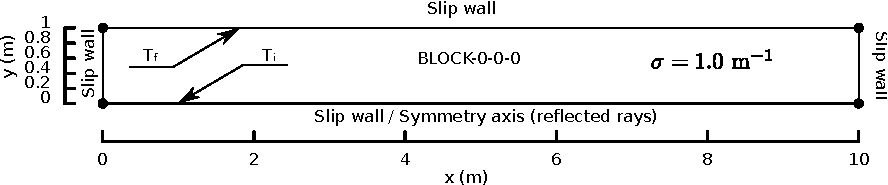
\includegraphics[width=\linewidth]{radiation/figures/grayslab_1B.pdf}
\caption{Single-block computational domains for the infinite-cylinder test case (not-to-scale).}
\label{fig:GS_domains}
\end{figure}

The computational domain for the test case is shown in Figure~\ref{fig:GS_domains}.
The present implementation of the ray-tracing algorithm only permits reflective boundary conditions along the $y = 0$ line; the east and west boundaries are therefore considered to be walls, rather than symmetry boundaries.
As will be demonstrated, however, the aspect ratio of 10:1 is sufficient to permit the infinite-slab and infinite-cylinder approximations at the slab mid-section ($x=5$\,m).
Grid resolutions of $8 \times 8$,  $16 \times 16$, $32 \times 32$ and $64 \times 64$ uniformly spaced cells are considered.
The cylinder is filled gas at a constant temperature of 10,000~K.
A `gray-gas' is assumed with a constant absorption coefficient of $\kappa$ = 1.0~m$^{-1}$, making the total emissive power density:

\begin{equation}
 j = \frac{\kappa \sigma T^{4}}{\pi}
 \label{eq:grey_emission}
\end{equation}


Although the radiation from a grey-gas can be described without considering spectral distributions, for this test case this is desirable so as to maintain similarity with the non-Planck spectra the model is designed to be applied to.
The spectral emission and absorption coefficients are then calculated as:

\begin{eqnarray}
      j_{\nu} &=& \kappa B_{\nu}(T) \\
 \kappa_{\nu} &=& \kappa 
\end{eqnarray}

\noindent where $B_{\nu}(T)$ is the Planck function:

\begin{equation}
 B_{\nu}(T) = \frac{2 h}{c^3} \frac{\nu^3}{e^\frac{h \nu }{k T} -1 }
\end{equation}

The spectral range considered is 10 to 3000\,nm, and is discretised with 500 intervals.
Integrating the Planck function with this discretisation matches the Stephan-Maxwell equation to within 0.1\%.
The exact solution for the axisymmetric test case is obtained from the analytical expressions presented by Sakai \textit{et al.}~\cite{SSM1998}.

\paragraph{Results}

Figure~\ref{fig:axi_divq_profiles} presents radiative divergence profiles at $x=5$\,m for the infinite-cylinder test case and a quantitative summary of the results are presented in Table~\ref{tab:axi_results}.
The quoted error in $\nabla \cdot \vec{q}_\text{rad}$ is the RMS of the absolute percentage difference along the $x=5$\,m profile referenced to the infinite-cylinder solution, and the quoted error in $q_\text{rad}$ is the average of the percentage difference from the infinite-cylinder solution at $3 \leq x \leq 7$\,m and $\tau_y=1$\,m.
All simulations were run using the serial version of the code on a single 2.2GHz AMD Opteron 6174 core of a Linux workstation with 132GB of RAM.
Note that more rays are required for the photon Monte-Carlo simulations as $N_\text{rays}$ is the total number of cells emitted per cell, whereas in the modified Discrete Transfer model $N_\text{rays}$ is the number rays emitted per cell \textit{per frequency interval}.

\begin{figure}[htb]
\centering
\subfloat[Modified Discrete Transfer model]{\scalebox{0.6}{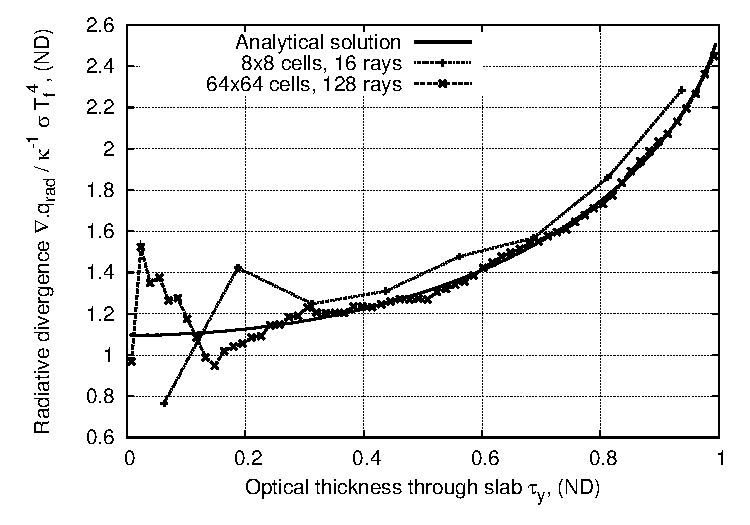
\includegraphics{radiation/figures/DT_divergence.pdf}}}
\subfloat[Photon Monte--Carlo model]{\scalebox{0.6}{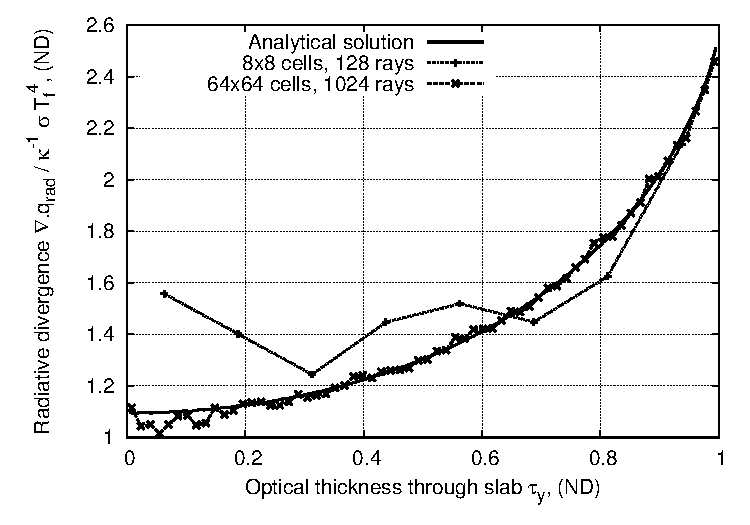
\includegraphics{radiation/figures/MC_divergence.pdf}}}
\caption{Comparison of radiative divergence solution profiles at $x=5$\,m for the axisymmetric infinite-cylinder radiation transport test case.}
\label{fig:axi_divq_profiles}
\end{figure}

\begin{table}[h]
 \centering
 \small
 \caption{Tabulated results for the axisymmetric infinite-cylinder radiation transport test case.}
 \label{tab:axi_results}
  \begin{threeparttable}
 \begin{tabular*}{0.95\textwidth}%
     {@{\extracolsep{\fill}}cccccc}
  \hline \hline \textbf{Grid Resolution}                                & \textbf{Ray resolution}      & \textbf{Memory}  &  \textbf{Wall time} & \textbf{RMS $\mathbf{\nabla \cdot \vec{q}_\text{rad}}$} & \textbf{$\mathbf{q_\text{rad}}$} \\
$\mathbf{(N_{\text{cells,x}}\times N_{\text{cells,y}})}$    & $\mathbf{N_\text{rays}}$  & \textbf{(MB)}        & \textbf{(s)}              & \textbf{Error (\%)}                                                      & \textbf{Error (\%)}                \\
\hline \multicolumn{6}{c}{\underline{Modified discrete transfer model}} \\
              $8 \times 8$                                                              & 16                                        &                                &   0.28                     &  10.71                                                                         & 4.32 \\
              $16 \times 16$                                                         &  32                                        &                                &  4.57                      & 4.54                                                                            & 2.51 \\
              $32 \times 32$                                                         & 64                                         &    290                     &  62.02                    & 6.49                                                                            & 1.65 \\
              $64 \times 64$                                                         & 128                                       &    3703                  &  1002.97                & 1.44                                                                            & 1.20 \\
\hline \multicolumn{6}{c}{\underline{Photon Monte-Carlo model}} \\
              $8 \times 8$                                                              & 128                                       &                                &  0.24                       &  14.78                                                                       & 4.10 \\
              $16 \times 16$                                                         &  256                                      &   13                         &  3.50                      & 1.18                                                                           & 1.22 \\
              $32 \times 32$                                                         & 512                                       &    54                        &  55.47                    & 3.57                                                                           & 1.34 \\
              $64 \times 64$                                                         & 1024                                     &    128                     &  921.34                  & 0.25                                                                           & 0.85  \\
 \hline
 \end{tabular*}
 \end{threeparttable}
\end{table}

Overall, the results demonstrate that both ray-tracing models converge towards the exact solution with increasing grid and ray resolution for axisymmetric geometries.
While the error in both $\nabla \cdot \vec{q}_\text{rad}$  and $q_\text{rad}$ drops for most successive grid refinements, this is not the case from the $16 \times 16$ to the $32 \times 32$ cell grid.
Such behaviour requires that a thorough grid resolution study is performed when implementing these models.
Of the two models, the photon Monte--Carlo model exhibits both superior accuracy per CPU-time and memory usage efficiency.
For example, for the $64 \times 64$ cell grid, both models have approximately the same wall time yet the Monte--Carlo model uses 29 times less memory and is almost 6 times more accurate in calculating $\nabla \cdot \vec{q}_\text{rad}$.
Furthermore, the photon Monte--Carlo model does not suffer from the Discrete Transfer models poor performance near the axis of symmetry.
This is due to the Monte--Carlo models statistical selection of photon trajectories, whereas the Discrete Transfer model considers a regular radiation sub-grid.

\par

Table~\ref{tab:slab_resource_usage} compares the computational resource usage for the $32 \times 32$ cell grid and 512 photon Monte--Carlo case run with the \verb OpenMP  version of the code using 1, 2 and 4 CPU cores of the same Linux workstation used for the resolution studies.
The results indicate the ray-tracing model performs reasonably well under parallelisation for simple grids.
The speed-ups for the 2 and 4 block cases are 1.52 and 2.97 respectively, giving parallelised code fractions of 48 and 34\% according to Gustafson's law~\cite{gustafson88}.
% Furthermore, the increase in the memory usage for the 2 and 4 core cases is minimal, being only 7.6 and 12.5\% respectively.

\begin{table}[b!]
 \centering
 \small
 \caption{Comparison of resource usage for the $32 \times 32$ cell grid and 512 photon Monte--Carlo infinite-cylinder radiation transport test case with 1, 2 and 4 blocks.}
 \label{tab:slab_resource_usage}
  \begin{threeparttable}
 \begin{tabular*}{0.95\textwidth}%
     {@{\extracolsep{\fill}}cccccc}
  \hline \hline \textbf{Number of CPU cores}, $\mathbf{N_\text{core}}$                          &  \textbf{Memory (MB)}  &  \textbf{Wall time (s)} &   \textbf{Speed up} \\
 \hline                                                    1                                                                                   & 54                                    &   55.47                         &  - \\
                                                               2                                                                                   & 119                                  &   36.45                         & 1.52 \\
                                                               4                                                                                   & 260                                  &   18.70                         & 2.97 \\
  \hline
 \end{tabular*}
 \end{threeparttable}
\end{table}
